\documentclass{standalone}
\usepackage{tikz}
% \usepackage{ifthen}
% \input{../include/flatland/flatland}
% \usetikzlibrary{shapes, arrows, positioning}
\begin{document}
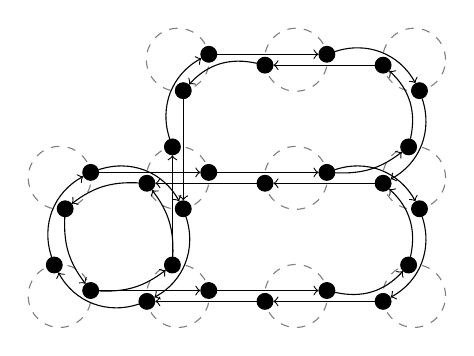
\begin{tikzpicture}[
  node distance=1.5cm,
  main/.style={circle, draw, dashed, minimum size=0.8cm, gray},
  sub/.style={circle, draw, fill=black, minimum size=0.2cm, inner sep=0pt}
  ]

  \node[main] (00) at (0,0) {};
  \node[main] (10) at (1.5,0) {};
  \node[main] (20) at (3,0) {};
  \node[main] (30) at (4.5,0) {};

  \node[main] (01) at (0,1.5) {};
  \node[main] (11) at (1.5,1.5) {};
  \node[main] (21) at (3,1.5) {};
  \node[main] (31) at (4.5,1.5) {};

  \node[main] (12) at (1.5,3) {};
  \node[main] (22) at (3,3) {};
  \node[main] (32) at (4.5,3) {};

  % sub-nodes based on original edge connections
  % positions: north=80º, west=170º, south=260º, east=-10º (350º)
  % for (0,0): edges to (1,0) east and (0,1) north
  \node[sub] (00e) at ([shift={(0.393,0.069)}]00) {}; % east (-10°)
  \node[sub] (00n) at ([shift={(-0.069,0.393)}]00) {}; % north (80°)

  % For (1,0): had edges to (0,0) [west], (2,0) [east], (1,1) [north]
  \node[sub] (10w) at ([shift={(-0.393,-0.069)}]10) {}; % west (170°)
  \node[sub] (10e) at ([shift={(0.393,0.069)}]10) {}; % east (-10°)
  \node[sub] (10n) at ([shift={(-0.069,0.393)}]10) {}; % north (80°)

  % For (2,0): had edges to (1,0) [west], (3,0) [east]
  \node[sub] (20w) at ([shift={(-0.393,-0.069)}]20) {}; % west (170°)
  \node[sub] (20e) at ([shift={(0.393,0.069)}]20) {}; % east (-10°)

  % For (3,0): had edges to (2,0) [west], (3,1) [north]
  \node[sub] (30w) at ([shift={(-0.393,-0.069)}]30) {}; % west (170°)
  \node[sub] (30n) at ([shift={(-0.069,0.393)}]30) {}; % north (80°)

  % For (0,1): had edges to (0,0) [south], (1,1) [east]
  \node[sub] (01s) at ([shift={(0.069,-0.393)}]01) {}; % south (260°)
  \node[sub] (01e) at ([shift={(0.393,0.069)}]01) {}; % east (-10°)

  % For (1,1): had edges to (0,1) [west], (2,1) [east], (1,0) [south], (1,2) [north]
  \node[sub] (11w) at ([shift={(-0.393,-0.069)}]11) {}; % west (170°)
  \node[sub] (11e) at ([shift={(0.393,0.069)}]11) {}; % east (-10°)
  \node[sub] (11s) at ([shift={(0.069,-0.393)}]11) {}; % south (260°)
  \node[sub] (11n) at ([shift={(-0.069,0.393)}]11) {}; % north (80°)

  % For (2,1): had edges to (1,1) [west], (3,1) [east]
  \node[sub] (21w) at ([shift={(-0.393,-0.069)}]21) {}; % west (170°)
  \node[sub] (21e) at ([shift={(0.393,0.069)}]21) {}; % east (-10°)

  % For (3,1): had edges to (2,1) [west], (3,0) [south], (3,2) [north]
  \node[sub] (31w) at ([shift={(-0.393,-0.069)}]31) {}; % west (170°)
  \node[sub] (31s) at ([shift={(0.069,-0.393)}]31) {}; % south (260°)
  \node[sub] (31n) at ([shift={(-0.069,0.393)}]31) {}; % north (80°)

  % For (1,2): had edges to (2,2) [east], (1,1) [south]
  \node[sub] (12e) at ([shift={(0.393,0.069)}]12) {}; % east (-10°)
  \node[sub] (12s) at ([shift={(0.069,-0.393)}]12) {}; % south (260°)

  % For (2,2): had edges to (1,2) [west], (3,2) [east]
  \node[sub] (22w) at ([shift={(-0.393,-0.069)}]22) {}; % west (170°)
  \node[sub] (22e) at ([shift={(0.393,0.069)}]22) {}; % east (-10°)

  % For (3,2): had edges to (2,2) [west], (3,1) [south]
  \node[sub] (32w) at ([shift={(-0.393,-0.069)}]32) {}; % west (170°)
  \node[sub] (32s) at ([shift={(0.069,-0.393)}]32) {}; % south (260°)

  \draw[thin] (10e) [<-] to[] (00e);
  \draw[thin] (20e) [<-] to[] (10e);

  \draw[thin] (20w) [<-] to[] (30w);
  \draw[thin] (10w) [<-] to[] (20w);
  \draw[thin] (10w) [<-] to[bend right=40] (11s);

  \draw[thin] (11e) [<-] to[] (01e);
  \draw[thin] (21e) [<-] to[] (11e);

  \draw[thin] (21w) [<-] to[] (31w);
  \draw[thin] (11w) [<-] to[] (21w);

  \draw[thin] (22e) [<-] to[] (12e);
  \draw[thin] (22w) [<-] to[] (32w);

  \draw[thin] (11n) [<-] to[] (10n);
  \draw[thin] (11s) [<-] to[] (12s);
  \draw[thin] (11s) [<-] to[bend right=40] (01e);

  \draw[thin] (01e) [<-] to[bend right=40] (00n);
  \draw[thin] (00e) [<-] to[bend left=20] (01s);


  \draw[thin] (12e) [<-] to[bend right=40] (11n);

  \draw[thin] (31w) [<-] to[bend left=30] (30n);
  \draw[thin] (30w) [<-] to[bend right=40] (31s);

  \draw[thin] (31w) [<-] to[bend right=40] (32s);
  \draw[thin] (32w) [<-] to[bend left=30] (31n);

  \draw[thin] (30n) [<-] to[bend left=30] (20e);
  \draw[thin] (00n) [<-] to[bend right=40] (10w);

  \draw[thin] (31n) [<-] to[bend left=20] (21e);
  \draw[thin] (31s) [<-] to[bend right=40] (21e);
  \draw[thin] (01s) [<-] to[bend left=20] (11w);
  \draw[thin] (32s) [<-] to[bend right=40] (22e);
  \draw[thin] (12s) [<-] to[bend left=30] (22w);
  \draw[thin] (10n) [<-] to[bend left=20] (00e);
  \draw[thin] (11w) [<-] to[bend left=20] (10n);

\end{tikzpicture}
\end{document}
%
%%% Local Variables:
%%% mode: LaTeX
%%% TeX-master: t
%%% End:
